\section{Collaborative ML Workload Optimizations} \label{sec-ml-workloads}
In this section, we present our collaborative ML workload optimization system.
Figure \ref{system-workflow} shows the architecture of our system, which comprises of a client and server component.
The client parses the user workload into a DAG (Step 1) and prunes the workload DAG (Step 2).
The server receives the workload DAG and utilizes our reuse algorithm to optimize the DAG (Step 3) and returns it to the client.
Finally, the client executes the optimized DAG (Step 4) and prompts the server to update the Experiment Graph and store the artifacts of the workload DAG (Step 5).
This architecture enables us to integrate our system into the existing collaborative environments without requiring any changes to their workflow.
The client and server can run within a single cloud environment where each client is an isolated container.
% In the rest of this section, we describe the process of parsing, pruning, generating workload DAGs, and executing the workloads.
% Then, we describe the process of constructing the Experiment Graph and how we utilize the Experiment Graph in our materialization and reuse algorithms. 
% Finally, we show the integration process and the impact of our system on our motivating example.
\subsection{Client Components}
\textbf{ML Script and Parser.}
We design an extensible DSL, which enables integration with Python data analysis and ML packages, such as Pandas \cite{mckinney-proc-scipy-2010} and scikit-learn \cite{sklearn_api}.
After invoking a script, the parser generates a DAG.
Listing \ref{listing-simple-workload} shows an example of a workload script.
The workload processes a dataset of ads description and trains a model to predict if an ad leads to a purchase.
% With only a slight modification of the import commands, we can load our parser modules.
Our system supports both long-running python scripts and interactive Jupyter notebooks.
\begin{figure}[t]
\centering
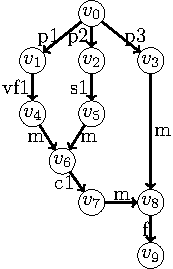
\includegraphics[width=\linewidth]{images/tikz-standalone/example-graph}
\caption{Workload DAG constructed from the Listing \ref{listing-simple-workload}. The highlighted node shows a terminal vertex.}
\label{fig-workload-dag}
\vspace{-5mm}
\end{figure}

\textbf{Workload DAG.}
In our DAG representation, vertices are the artifacts, i.e., raw or preprocessed data and ML models, and edges are the operations.
A workload DAG has one or more source vertices representing the raw datasets.
A workload DAG also contains one or more terminal vertices.
Terminal vertices are the output of the workload.
For example, a terminal vertex is a trained ML model or aggregated data for visualization.
Requesting the result of a terminal vertex triggers the optimization and execution of the workload DAG.
Figure \ref{fig-workload-dag} shows the workload DAG constructed of the code in Listing \ref{listing-simple-workload}.
In the Figure, the terminal vertex is the result of the print statement on Line 16 in Listing \ref{listing-simple-workload}.
\begin{lstlisting}[language=Python, caption=Example script,captionpos=b,label = {listing-simple-workload}]
import wrapper_pandas as pd
from wrapper_sklearn import svm
from wrapper_sklearn.feature_selection import SelectKBest
from wrapper_sklearn.feature_extraction.text import CountVectorizer

train = pd.read_csv('train.csv')  # [ad_desc,ts,u_id,price,y]
ad_desc = train['ad_desc']
vectorizer = CountVectorizer()
count_vectorized = vectorizer.fit_transform(ad_desc)
selector =  SelectKBest(k=2)
t_subset = train[['ts','u_id','price']]
y =  train['y']
top_features = selector.fit_transform(t_subset, y)
X = pd.concat([count_vectorized,top_features], axis = 1)
model = svm.SVC().fit(X, y)
print model # terminal vertex
\end{lstlisting}

\textbf{Local Pruner.}
Once the user requests the result of a terminal vertex, the client prunes the DAG before sending it to the server.
The pruner identifies edges that are not in the path from source to terminal and edges with their endpoint vertex already computed.
% The task of the pruner is to identify all the unnecessary edges.
% There are two groups of unnecessary edges: edges that are not in the path from source to terminal and edges with their endpoint vertex already computed.
The latter is very common in interactive workloads since every cell invocation in Jupyter notebooks computes some of the vertices.
As a result, in the future cell invocations, previously executed operations can be skipped.
Note that the pruner does not remove the edge from the DAG and only marks them as inactive.
For example, in Figure \ref{fig-workload-dag}, if \textit{t\_subset} is computed, the local pruner marks the edge between \textit{train} and \textit{t\_subset} as inactive.
After the pruning, the client sends the DAG to the server.
% To minimize the transfer cost, the client does not send the content of the computed artifact to the server.

\textbf{Executor.}
After the server optimizes a workload DAG, the executor receives the optimized DAG to execute the operations and returns the result to the user.
The executor runs the operations in the optimized DAG in their topological order and returns the result to the user.
% To avoid redundant computation, the executor ignores inactive edges.
After the executor completes the execution of a workload DAG, it annotates the DAG vertices with compute-time and sizes before sending it to the updater for storage.
\begin{figure}[t]
\centering
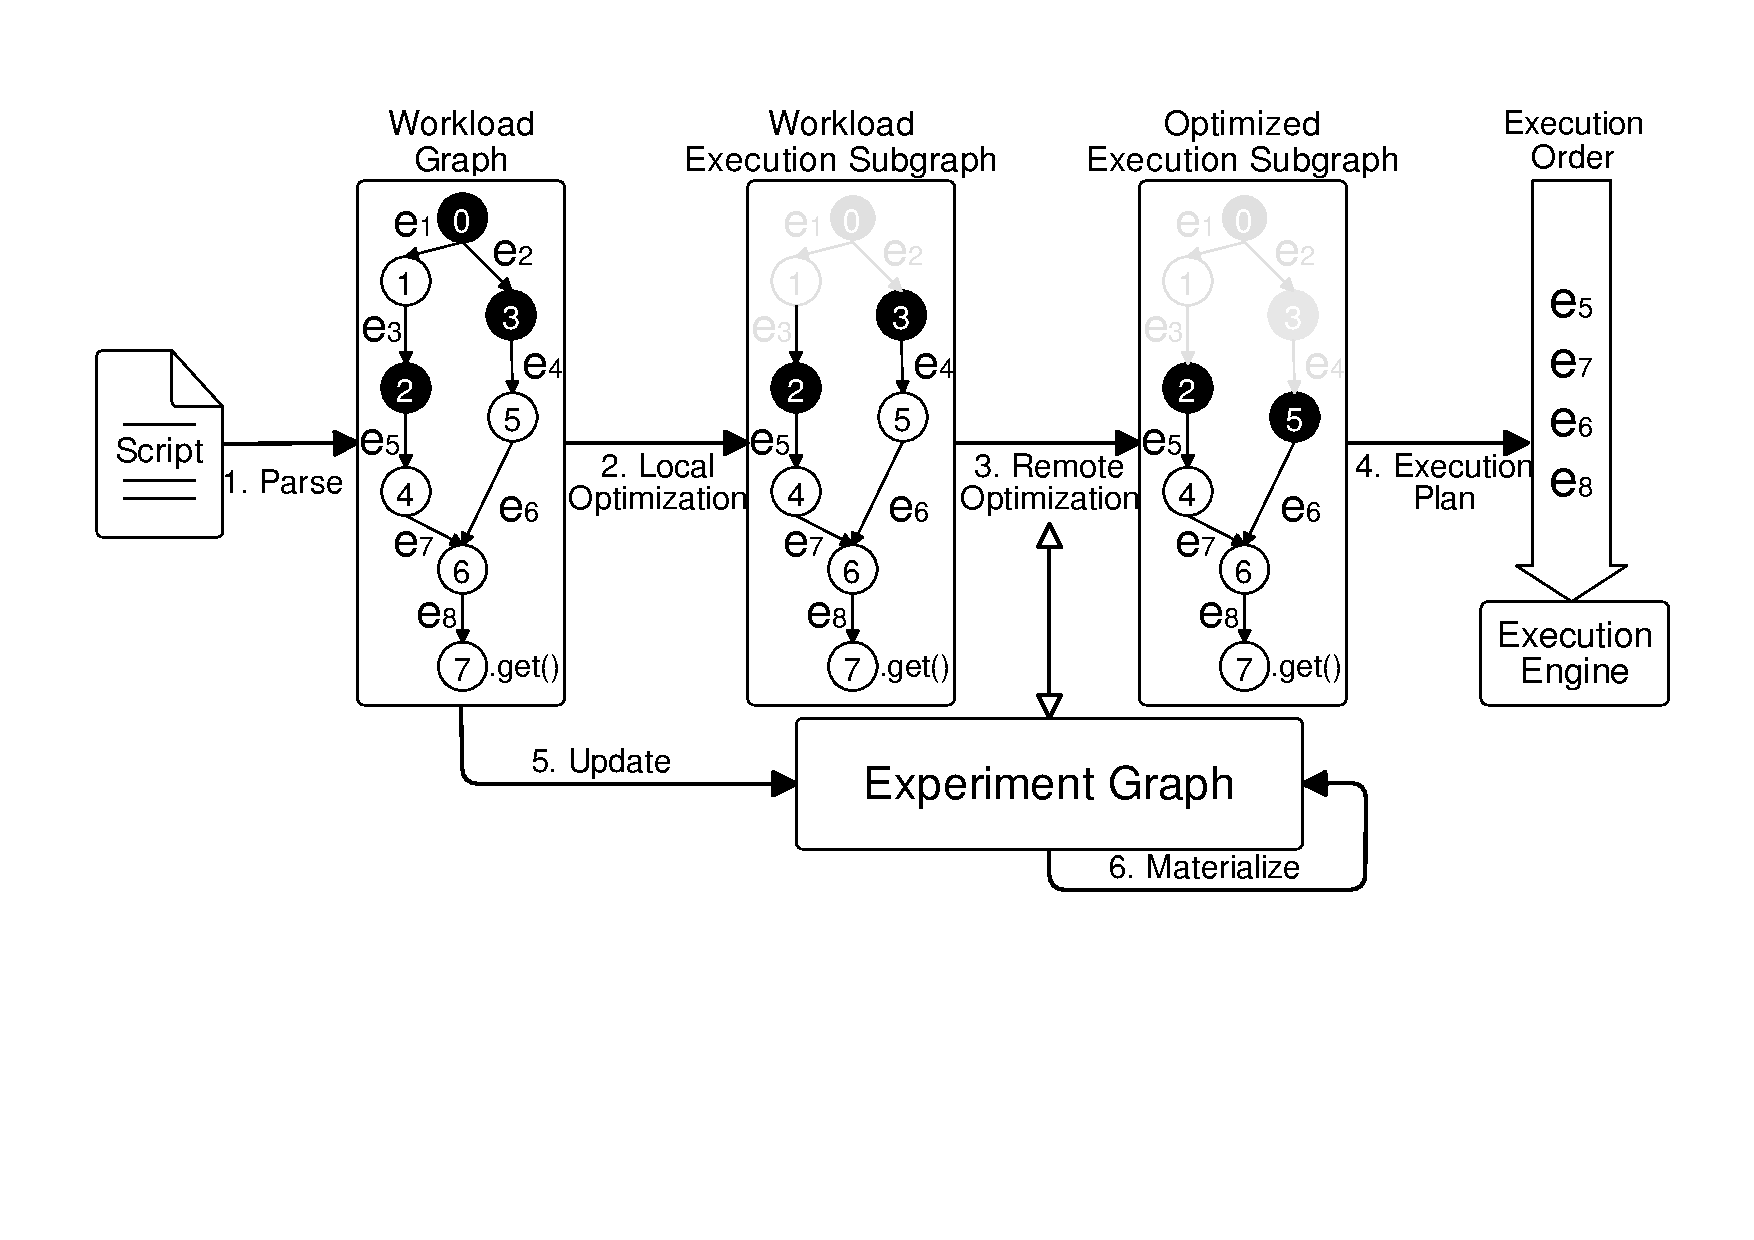
\includegraphics[width=0.9\columnwidth]{images/system-workflow}
\caption{Collaborative workload optimizer system}
\label{system-workflow}
\vspace{-5mm}
\end{figure}
\subsection{Server Components}
\textbf{Experiment Graph (EG).}
EG is the union of all the executed workload DAGs, where vertices represent the artifacts and edges represent the operations.
Every vertex in EG has the attributes $frequency$, $size$, and $compute\_time$, representing the number of workloads an artifact appeared in, the storage size, and the compute-time of the artifact, respectively.
Every vertex in EG carries the meta-data of the artifact it represents.
For datasets, the meta-data includes the name, type, and size of the columns.
For ML models, the meta-data includes the name, type, hyperparameters, and the evaluation score of the model.
To save storage space, EG does not contain the content, i.e., underlying data and model weights, of all the artifacts.
The updater component decides whether to store the content of an artifact.

EG maintains a list of all the source vertices that it contains.
Furthermore, every edge in the graph stores the hash of the operation it represents.
Therefore, given a workload DAG, EG quickly detects if it contains the artifacts of the workload DAG by traversing the edges starting from the source.
%Note that EG comprises of many connected components.
%Each connected component represents the union of all the workload DAGs that share the same source datasets and are solving the same machine learning task.
%In our motivating example, if one EG represents the entire Kaggle, each competition inside Kaggle is one connected component of EG.
%In the rest of the paper, when we use the term EG, we refer to one connected component.

\textbf{Optimizer. }
The optimizer receives the workload DAG from the client and queries EG for materialized artifacts.
Then, the optimizer utilizes our reuse algorithm to generate an optimized DAG by retrieving the optimal subset of the materialized vertices from EG.
The optimized DAG guarantees to incur the smallest cost, i.e., the transfer cost of the materialized artifacts plus execution cost of the operations.

\textbf{Updater.}
The updater receives the executed DAG from the client.
The vertices in the executed DAG contain the size and compute-time of the artifacts they represent.
The updater performs the three following tasks.
First, it stores any source artifact, both the meta-data and the content, that is not in EG.
This is to ensure that EG contains every raw dataset.
Second, it updates EG to include all the vertices and edges of the executed DAG.
If EG already contains a vertex, the updater increases its frequency.
Lastly, by utilizing our novel materialization algorithms, the updater stores the content of a selected set of artifacts, i.e., the output of the materialization algorithms.
Note that EG contains the meta-data of all the artifacts, including the unmaterialized artifacts.
\subsection{Improved Motivating Example}
By utilizing our collaborative workload optimizer, we can improve the execution of the workloads in our motivating example.
We maintain an EG for the Home Credit Default Risk competition.
After users publish their workload scripts on Kaggle, other users will read, re-run, or modify the scripts.
The updater component of our system stores the artifacts with a high likelihood of reuse into EG.
Our optimizer generates efficient workloads by querying EG for materialized artifacts and transforming the workload DAG into a more optimized DAG.
We highlighted three workloads that were copied and modified 7000 times.
Optimizing these workloads saves hundreds of hours of execution time, which reduces the required resources and operation cost of Kaggle.